%%
%% This is file `sample-sigconf-authordraft.tex',
%% generated with the docstrip utility.
%%
%% The original source files were:
%%
%% samples.dtx  (with options: `all,proceedings,bibtex,authordraft')
%% 
%% IMPORTANT NOTICE:
%% 
%% For the copyright see the source file.
%% 
%% Any modified versions of this file must be renamed
%% with new filenames distinct from sample-sigconf-authordraft.tex.
%% 
%% For distribution of the original source see the terms
%% for copying and modification in the file samples.dtx.
%% 
%% This generated file may be distributed as long as the
%% original source files, as listed above, are part of the
%% same distribution. (The sources need not necessarily be
%% in the same archive or directory.)
%%
%%
%% Commands for TeXCount
%TC:macro \cite [option:text,text]
%TC:macro \citep [option:text,text]
%TC:macro \citet [option:text,text]
%TC:envir table 0 1
%TC:envir table* 0 1
%TC:envir tabular [ignore] word
%TC:envir displaymath 0 word
%TC:envir math 0 word
%TC:envir comment 0 0
%%
%% The first command in your LaTeX source must be the \documentclass
%% command.
%%
%% For submission and review of your manuscript please change the
%% command to \documentclass[manuscript, screen, review]{acmart}.
%%
%% When submitting camera ready or to TAPS, please change the command
%% to \documentclass[sigconf]{acmart} or whichever template is required
%% for your publication.
%%
%%
\documentclass[sigconf,10pt]{acmart}
%%
%% \BibTeX command to typeset BibTeX logo in the docs
\AtBeginDocument{%
  \providecommand\BibTeX{{%
    Bib\TeX}}}

%% Rights management information.  This information is sent to you
%% when you complete the rights form.  These commands have SAMPLE
%% values in them; it is your responsibility as an author to replace
%% the commands and values with those provided to you when you
%% complete the rights form.
\setcopyright{acmlicensed}
\copyrightyear{2018}
\acmYear{2018}
\acmDOI{XXXXXXX.XXXXXXX}
%% These commands are for a PROCEEDINGS abstract or paper.
\acmConference[Conference acronym 'XX]{Make sure to enter the correct
  conference title from your rights confirmation email}{June 03--05,
  2018}{Woodstock, NY}
%%
%%  Uncomment \acmBooktitle if the title of the proceedings is different
%%  from ``Proceedings of ...''!
%%
%%\acmBooktitle{Woodstock '18: ACM Symposium on Neural Gaze Detection,
%%  June 03--05, 2018, Woodstock, NY}
\acmISBN{978-1-4503-XXXX-X/2018/06}


%%
%% Submission ID.
%% Use this when submitting an article to a sponsored event. You'll
%% receive a unique submission ID from the organizers
%% of the event, and this ID should be used as the parameter to this command.
%%\acmSubmissionID{123-A56-BU3}

%%
%% For managing citations, it is recommended to use bibliography
%% files in BibTeX format.
%%
%% You can then either use BibTeX with the ACM-Reference-Format style,
%% or BibLaTeX with the acmnumeric or acmauthoryear sytles, that include
%% support for advanced citation of software artefact from the
%% biblatex-software package, also separately available on CTAN.
%%
%% Look at the sample-*-biblatex.tex files for templates showcasing
%% the biblatex styles.
%%

%%
%% The majority of ACM publications use numbered citations and
%% references.  The command \citestyle{authoryear} switches to the
%% "author year" style.
%%
%% If you are preparing content for an event
%% sponsored by ACM SIGGRAPH, you must use the "author year" style of
%% citations and references.
%% Uncommenting
%% the next command will enable that style.
%%\citestyle{acmauthoryear}

%\usepackage{todonotes}
\usepackage{booktabs}
\usepackage{multirow}
 \usepackage{proof}
\usepackage{array}
\newcolumntype{O}[1]{>{\raggedright\arraybackslash}m{#1}}
\newcolumntype{P}[1]{>{\centering\arraybackslash}m{#1}}
\newcolumntype{Q}[1]{>{\raggedleft\arraybackslash}m{#1}}
\newcolumntype{S}{>{\centering\arraybackslash}m{2cm}}
% Useful macros from Isaac Oscar Gariano: a very simple library for author-specific change notations:
%  After calling \newAuthor{<name>}{<colour>}
% You can use \<name>{<text>} to add a comment
% Or \<name>A{<text>} to  write stuff in your colour (to denote additional text)
% Or \<name>B{<text>} is similar, but changes the background (to highlight stuff?)
% I may add more commands later
% (there's a 'changes' package with similar functionality, but it has a habit of breaking when you use it with  the Define environment)
\newcommand\newAuthor[2]{%
        \ExpandArgs{c}\newcommand{#1}[1]{\todo[color=#2!10, bordercolor=#2, inline]{\textbf{#1:}~##1}}
	\ExpandArgs{c}\newcommand{#1A}[1]{\textcolor{#2}{##1}}
        \ExpandArgs{c}\newcommand{#1B}[1]{\colorbox{#2!30}{\textcolor{black}{##1}}}}
\newtheorem*{remark}{Remark}
\newcommand{\blackdiamond}{\rotatebox[origin=c]{45}{$\vcenter{\hbox{$\scriptscriptstyle\blacksquare$}}$}}

\newAuthor{Ismail}{blue}
\newAuthor{Colin}{cyan}

%% The "title" command has an optional parameter,
\usepackage{amsthm}
\theoremstyle{definition}
\newtheorem{definition}{Definition}[section]
%%
%% end of the preamble, start of the body of the document source.
\begin{document}

%%
%% The "title" command has an optional parameter,
%% allowing the author to define a "short title" to be used in page headers.
\title{On Verification Patterns for Low-Level Systems via Modal Abstractions }

%%
%% The "author" command and its associated commands are used to define
%% the authors and their affiliations.
%% Of note is the shared affiliation of the first two authors, and the
%% "authornote" and "authornotemark" commands
%% used to denote shared contribution to the research.
% Commentout
%\author{Ben Trovato}
%\authornote{Both authors contributed equally to this research.}
%\email{trovato@corporation.com}
%\orcid{1234-5678-9012}
%\author{G.K.M. Tobin}
%\authornotemark[1]
%\email{webmaster@marysville-ohio.com}
%\affiliation{%
 % \institution{Institute for Clarity in Documentation}
 % \city{Dublin}
 % \state{Ohio}
 % \country{USA}
%}

%%
%% By default, the full list of authors will be used in the page
%% headers. Often, this list is too long, and will overlap
%% other information printed in the page headers. This command allows
%% the author to define a more concise list
%% of authors' names for this purpose.
\renewcommand{\shortauthors}{Kuru and Gordon}

%%
%% The abstract is a short summary of the work to be presented in the
%% article.
\begin{abstract}
 Although they differ in the functionality they offer, low-level systems exhibit certain patterns of design and utilization of computing resources.

  In this paper, we argue the position that \emph{modalities}, in the sense of modal logic, 
  should be a go-to approach when specifying and verifying low-level systems code.
  We explain how the concept of a \emph{resource context} helps guide the design of new modalities
  for verification of systems code, and
  we justify our perspective by discussing prior systems that have used modalities for systems verification
  successfully, arguing that they fit into the verification design pattern we articulate,
  and explaining how this approach might apply to other systems verification challenges.
\end{abstract}

%%
%% The code below is generated by the tool at http://dl.acm.org/ccs.cfm.
%% Please copy and paste the code instead of the example below.
%%
%\begin{CCSXML}
%<ccs2012>
% <concept>
%  <concept_id>00000000.0000000.0000000</concept_id>
%  <concept_desc>Do Not Use This Code, Generate the Correct Terms for Your Paper</concept_desc>
%  <concept_significance>500</concept_significance>
% </concept>
% <concept>
%  <concept_id>00000000.00000000.00000000</concept_id>
%  <concept_desc>Do Not Use This Code, Generate the Correct Terms for Your Paper</concept_desc>
%  <concept_significance>300</concept_significance>
% </concept>
% <concept>
%  <concept_id>00000000.00000000.00000000</concept_id>
%  <concept_desc>Do Not Use This Code, Generate the Correct Terms for Your Paper</concept_desc>
%  <concept_significance>100</concept_significance>
% </concept>
% <concept>
%  <concept_id>00000000.00000000.00000000</concept_id>
%  <concept_desc>Do Not Use This Code, Generate the Correct Terms for Your Paper</concept_desc>
%  <concept_significance>100</concept_significance>
% </concept>
%</ccs2012>
%\end{CCSXML}
%
%\ccsdesc[500]{Do Not Use This Code~Generate the Correct Terms for Your Paper}
%\ccsdesc[300]{Do Not Use This Code~Generate the Correct Terms for Your Paper}
%\ccsdesc{Do Not Use This Code~Generate the Correct Terms for Your Paper}
%\ccsdesc[100]{Do Not Use This Code~Generate the Correct Terms for Your Paper}
%
%%%
%%% Keywords. The author(s) should pick words that accurately describe
%%% the work being presented. Separate the keywords with commas.
%\keywords{Do, Not, Us, This, Code, Put, the, Correct, Terms, for, Your, Paper}
%% A "teaser" image appears between the author and affiliation
%% information and the body of the document, and typically spans the
%% page.
%\begin{teaserfigure}
%  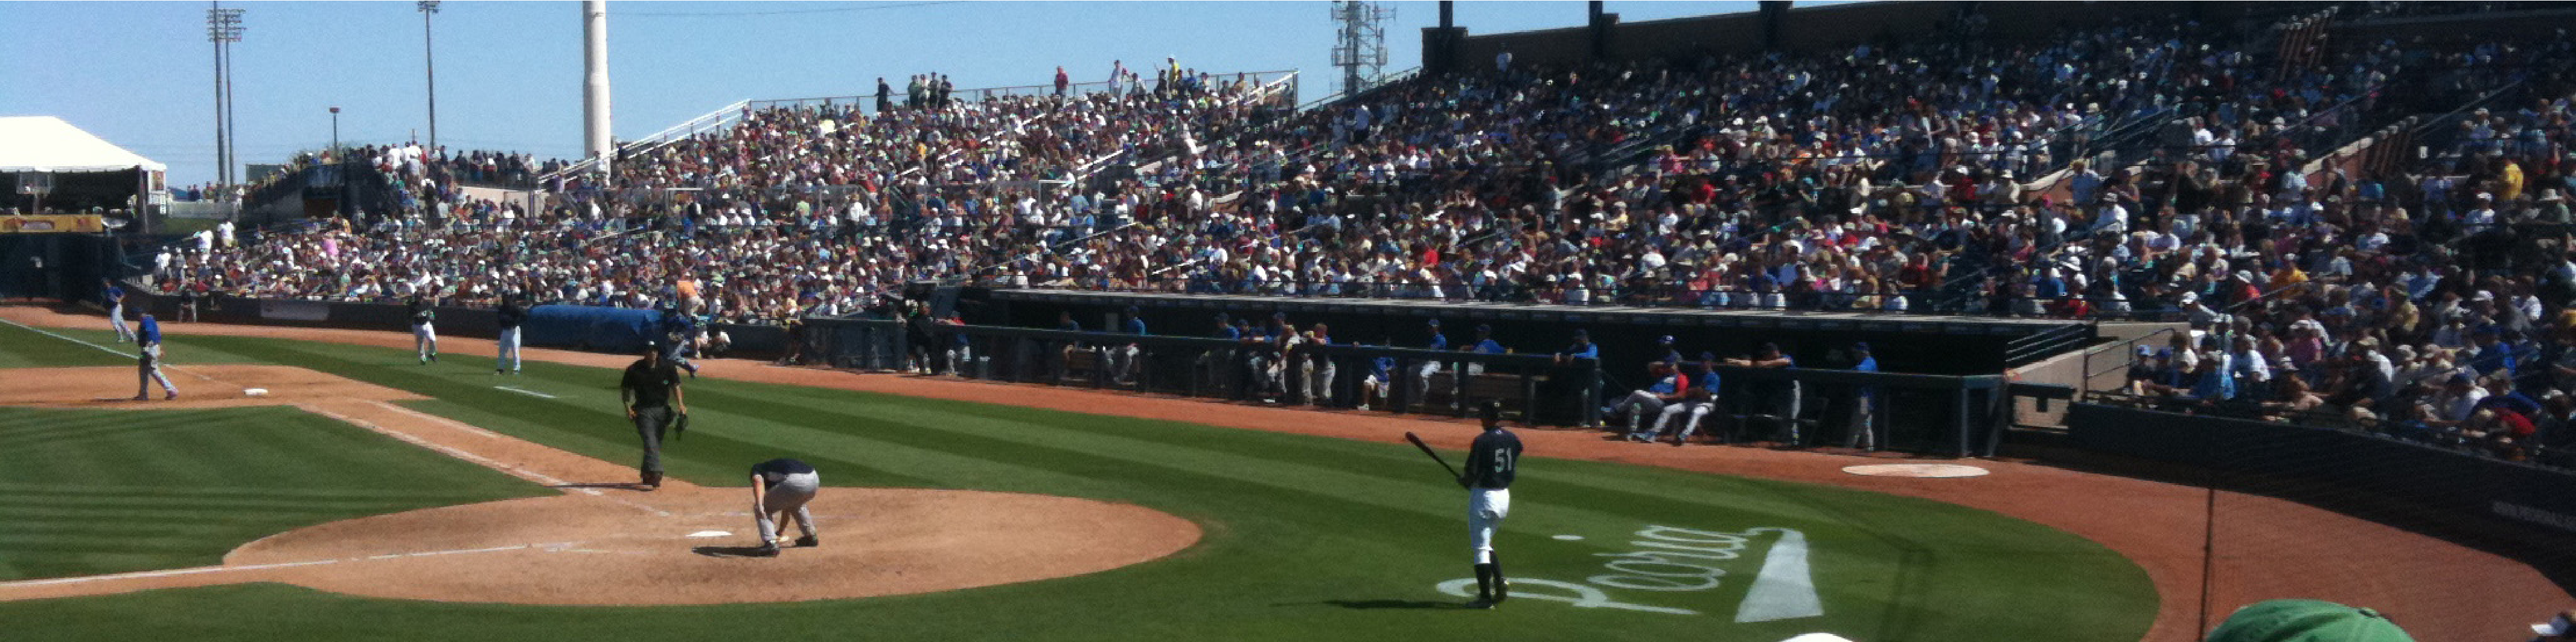
\includegraphics[width=\textwidth]{sampleteaser}
%  \caption{Seattle Mariners at Spring Training, 2010.}
%  \Description{Enjoying the baseball game from the third-base
%  seats. Ichiro Suzuki preparing to bat.}
%  \label{fig:teaser}
%\end{teaserfigure}

%\received{20 February 2007}
%\received[revised]{12 March 2009}
%\received[accepted]{5 June 2009}

%%
%% This command processes the author and affiliation and title
%% information and builds the first part of the formatted document.
\maketitle
\section{Introduction}
\label{sec:intro}
Systems verification has attracted much attention from both the verification community and the systems community over the past couple of decades. %There are two main streams of verification efforts on systems. In one class of verification, \emph{automated} verification tools are used. They allow people to specify systems via specific annotation languages they offer, and incorporate translation of these specifications into SMT-like formulas for which proofs are searched by the SMT solvers at the backend ~\cite{}. 
Most of this effort has been build on top of \emph{program logics}~\cite{reynolds2002separation,hoare1969axiomatic,smans2012implicit,pratt1976semantical},
which are formal logics of reasoning about program behaviour --- given any starting state
satisfying a particular precondition, running a certain code segment of interest should not fail and should produce a final state satisfying a desired postcondition.
This requires an interacting family of pieces, including a specification language
to describe those desired pre- and postconditions, as well as rules of the logic to deal with
how program operations like variable or register assignments and memory accesses interact with pre- and postconditions.
Since most low-level systems are stateful, \emph{separation logic} has been the focus 
of most recent work.
%has been either the foundational or direct choice of logic in these verification efforts. 
%\Colin{Talking about separation logic makes lots of sense. Do we care about Iris/Coq/Lean/etc. vs. automation? Using the modality idea
%for something like Dafny would certainly look different from the Iris work, but can't it work?
%e.g. \url{https://csgordon.github.io/publications/agere19/}
%I don't want to push to plug my own work if you don't think it makes sense or are making a different point. But I think it's worth
%considering how broadly the big ideas can be applied.
%}

%Advancements in separation logic have been drastic ~\cite{}. These advancements, such as the capability of introducing \emph{ghost} (logical) bookkeeping and associating this bookkeeping with the concept of \emph{invariant} in Iris separation logic, increased the expressivity of any logic that is built on top. Expectedly, many logics enjoying these strong \emph{separation logic} capabilities have been built to verify low-level systems~\cite{}.  %All these program logics built on top of Iris customize and utilize two main aspects of a separation logic like Iris.
%%\paragraph{Custom-Tailored Weakest-Precondition (WP)}
%%\todo[inline]{speak about crash modality etc, encoding how the state should get changed ... GC as well}
%%\paragraph{An Essential Step in Operational Semantics}
%%\todo[inline]{speak about crash step in operational semantics. GC as well}
%%Regarding generalization of customized weakest-preconditions, there has been foundational generalizations defined over incorporating the knowledge of how the resources change, i.e.,transformation of resources, ~\cite{nextgenmodality}, into the separation logic resource assertions. This allows encoding the many customized weakest-preconditions as an instance of a generalized modality definition and lifting of the composition of resource transformation knowledge, which itself is defined as a resource algebra, to the ordinary separation logic resource assertions so that all the underlying resource algebra capabilities can be used for the assertions decorated with the resource-transformation modality. However, even with this kind of generalization effort, it still customizes both the weakest-precondition and resource assertions with the version value (\emph{transformation-generation} value) which most probably lacks being generalizable regarding the real systems to be specified with it as it is not always the case that systems take \emph{versioning} as its key aspect. In general, modalities used in program verification ~\cite{}, are either still tightly coupled with the separation logic they are hosted in, i.e., modalities as definitions for hiding which state a certain truth on resources holds, or as part of the underlying logic's machinery, e.g., later modality as logical machinery encoding step-indexing mechanism.
Modern separation logics are often implemented as frameworks (notably \textsc{Iris}~\cite{jung2018iris}), which offers a collection of tools for building custom separation logic variants for resources of interest, modularly. This makes it possible to
reuse significant amounts of work across verifications using memory~\cite{jung2018iris},
disks~\cite{chajed2019verifying}, and other diverse resources.
%Highly customizable logic ~\cite{iris,..} being the basis for building custom-tailored logics for specific verification tasks ~\cite{some sl refs} enabled building clean and intuitive specifications and proof rules. 
When not using such a framework and instead using an existing tool~\cite{leino2010dafny,vazou2014refinement} as a basis, one can often customize the assertion language by defining libraries of specification definitions and lemmas to effectively have a custom logic.

With these options comes the question: if you can customize your verification tool and how it expresses program states, \emph{how should} you customize it?
We argue that a go-to methodology should be to define \emph{modalities},
which it turns out are in active use in a variety of systems papers because that approach seems to naturally fit many problems that arise in verifying systems code
~\cite{tejperennial19,tejthesis, derekrustbelt20, jung2018iris, kuru2024modalabstractionsvirtualizingmemory, garbagecollect, amalreal2024,fsl, fsl++}.

This paper  
 \begin{itemize}
 \item builds an intuition from a systems-verification perspective about the modal concepts that have been used in recent years with modern program logic -- Section \ref{sec:motivation}
\item describes the common structure underlying the modalities used in systems verification work, effectively a high-level design pattern and process for designing a customized specification language, which has not previously been described --- Section \ref{sec:definitions} % to understand the structure of modal abstractions given for different kinds of systems in Table \ref{table:decomposition}
%\item identifies the common patterns in different modal abstractions for different systems
\item gives example specifications to critical steps of different systems, and discuss how modal abstractions look in these specifications
\end{itemize}

\section{Motivation, Background, and Related Work}
\label{sec:motivation}
To explain our ideas clearly, we briefly recap some of the background and themes our ideas build on,
casting them in a certain way to bring out the relevance of our philosophy.
%\begin{table}[h]
%\centering
%\caption{Decomposing Systems}
%\label{table:decompositionsys}
%\begin{tabular}{@{}lcScP{2cm}@{}}
%\toprule
%   & Column & Column                    & Column                   & Column \\ \midrule
%Row & 1      & 2                         & 3                        & $k=a+b+c+d+e+f+g$      \\
%Row & 5      & \multicolumn{2}{c}{\multirow{2}{*}{Because why not}} & 8      \\
%Row & 9      & \multicolumn{2}{c}{}                                 & 12     \\
%Row & 13     & $k=a+b+c+d+e$                        & 15                       & 16     \\ \bottomrule
%\end{tabular}
%\end{table}

\subsection{Resources in Systems Software}
\label{sec:systemsoft}
Systems software, in general, interfaces with an underlying computing architecture such that any software system at any higher level in the software stack can (at least indirectly) utilize the resources of the machine.
The last layer of software before the hardware is naturally critical to the correctness of an overall system,
as essentially all software built on top of it assumes its correctness.
%Assuming verified hardware, this makes the correctness of the system software critical to the rest of the software stack. 
%Because they interface with the hardware, abstractions and their implementations are intricate and error-prone. 
And because hardware is complex and highly diverse, the implementation of those lowest layers
of the software stack is typically intricate and naturally error-prone, despite how critical its correctness is.
Typically systems software has, as a primary focus, the task of \emph{abstracting} from hardware details to simplify 
the construction of higher layers of the stack.

\paragraph{Virtualization}
One of the most common forms of abstraction provided by systems software is \emph{virtualization},
which abstracts the relationship between conceptual and physical computing resources. 
Operating System (OS) kernels virtualize memory locations and quantity (via virtual memory and paging~\cite{denning1970virtual}).
Distributed language runtimes may virtualize addresses, even when processes may migrate across machines~\cite{jul1988fine}.
Filesystems virtualize locations on disk~\cite{rodeh2013btrfs,hitz1994file,rosenblum1992design,bonwick2003zettabyte}.
Programs built on top of the corresponding systems software layer work logically at the level of these virtualized resources,
and it makes sense to specify the systems software directly in terms of those abstractions.

\paragraph{Sharing} is one of the fundamental reasons for kernels to {virtualize} resources,
for creating the illusion of exclusive access to virtualized versions of shared resources, including CPU time (via preemption).
An implementation of sharing relies on two concepts: \emph{indirection} and \emph{coordination}. Indirection is a method that allows the mapping of resources of one type into another. By doing so, it allows treating the limited resources (e.g. hardware resources such as physical memory) as if there are more than they actually are (e.g. via virtual memory addresses and paging). Consequently, virtualization for the sake of ensuring availability requires \emph{sharing} of the resources that exist in reality.

\paragraph{Access by Translation}
Accessing virtualized resources via translation is a common way to virtualize notions of location (e.g.,
virtual memory addresses, inodes or object IDs instead of disk addresses~\cite{bonwick2003zettabyte,hitz1994file,rosenblum1992design,rodeh2013btrfs}).
%Accessing the hardware resources in the presence of sharing means having more resource references (references to the virtualized resources) to access the \emph{mapped} resources that are physical and potentially fewer. 
B-trees~\cite{}, page tables~\cite{}, and related structures both behave like maps, when the corresponding physical resources exist as such
just in a different location.
Control over the lookup process (e.g, handling the case of a missing translation entry) allows for additional flexibility,
such as filling holes in sparse files, or demand paging (both from disk or lazily populating anonymous initially-zeroed mappings).
Although the realization of these maps may differ from a system to system based on the context (and sometimes hardware details),
they are semantically --- logically --- partial maps, worth treating as such in verification. 

%\paragraph{Isolation Hand-in-Hand with Sharing}
%\Ismail{put a few words on abstractions such as address space, stack region, snapshots ,etc.}
%\Colin{Not sure what you want here?}

\subsection{Logic of Resources \& Systems Verification }
\label{sec:seplogic}
Separation logic~\cite{reynolds2002separation} is a specialization of Hoare Logic~\cite{hoare1969axiomatic}
to better deal with reasoning about disjoint resources.
Classic Hoare Logic, as used in prominent systems verifications like \textsc{seL4}~\cite{klein2014comprehensive},
deals with pre- and post-conditions. A so-called ``triple''
\[
\{P\}\;C\;\{Q\}
\]
represents an assertion that if the current program state is accurately described by assertion $P$,
then executing the ``command'' (program) $C$ will not crash, and if it terminates then $Q$ will accurately
describe the ending program state.

\paragraph{Ownership} Separation Logic extends Hoare Logic 
with an additional logical connective $\ast$ (called \emph{separating conjunction}) such that $P \ast Q$ asserts that $P$ and $Q$ not only both hold, but apply to
\emph{disjoint} portions of the program state.\footnote{Though much like systems design, modern separation logics~\cite{jung2018iris}
allow this separation to apply to a kind of virtualization of physical resources~\cite{jensen2012fictional},
or even resources that only exist in the logic~\cite{jung2016higher}.
}
This disjointness assumption leads to discussing separation logic assertions as asserting \emph{ownership}
of the (physical or virtual) resources they hold on.
The classic \emph{points-to} assertion $\ell\mapsto v$ asserts ownership of a portion of memory containing memory address
$\ell$, and that the memory at that location contains value $v$. The disjointness from separating conjunction
is useful: if $\ell\mapsto v \ast \ell'\mapsto v'$ is true, it means $\ell$ and $\ell'$ are distinct memory addresses,
because they must hold on disjoint parts of memory.

Modern separation logics~\cite{jung2018iris} allow definition of more nuanced versions of this idea.
A common form of this, which we revisit in Section \ref{sec:definitions}, is the parameterization of this and
other assertions by a kind of context --- a \emph{resource context} --- resulting in assertions like  $\ell \mapsto_{\textsf{Ctx}} v$, conveying the ownership of the resource defined by the reference $\ell$ and the value ($v$) it's referring to, but where the \emph{resource context}
of the assertion may have the name ($\ell$) and value ($v$) exist not in a partial map of physical memory locations to values,
but of register names to register values~\cite{chlipala2011mostly,ni2007using},
filesystem block indices to block contents~\cite{chajed2019verifying},
or other kinds of associations.
Thus much of the machinery of modern separation logics comes from shifting the notion of which resource context 
assertions are relative to.

%\Colin{Regarding next paragraph: separation logics are not necessarily foundational (early work was all pen-and-paper,
%automated work with SMT solvers clearly isn't foundational). Unless you mean ``foundational'' in a non-technical sense (in which case, a different word should be used, to avoid confusion).}
%\paragraph{Specification} Separation logics~\cite{} rely on foundational Hoare-Logic when introducing their abstractions: make specific assertions and abstractions appear in the form of pre- and post-conditions, $\{P\} e \{Q\}$, called Hoare Triple. It is also important to note that program logics also enjoy encoding Hoare Triples in terms of weakest-precondition~\cite{dijkstra1975guarded} program logics~\cite{pratt1976semantical}, which is roughly
%\[\textsf{P} \; -\ast \;\textsf{wp}\; e \; \{Q\}\]
%where $-\ast$ can  be intuitively thought of as \textit{"when P is added into the resource context we can have the resource represented with Q"}
%\Colin{\emph{Is} it important to note this? I'm genuinely not sure it is.}

\subsection{Modal Reasoning}
\label{sec:modalbackground}
Modal logics are logics of contingent truth, enabling reasoning about cases where something is or may
be true in alternate circumstances. These alternate circumstances are expressed via modal operators,
which decorate a proposition with those alternate circumstances of its truth. This can be express
conditions related to time~\cite{pnueli1977temporal} (e.g., $\diamond P$ for $P$ being true at some point in the future in \textsc{LTL}), necessity and/or possibility~\cite{harel1979first,pratt1976semantical} (e.g., $[C]P$ indicating that $P$ is true after execution
of the program command $C$ terminates), or knowledge and belief~\cite{halpern1990knowledge,hintikka1962knowledge}
(e.g., $\mathcal{K}_a P$ indicating that node $a$ in a distributed system possesses knowledge of $P$),
or the location \emph{where} something is true~\cite{murphy2007type,gordon2019modal}.

\paragraph{Nominals} 
Some classes of assertions benefit specifically from \emph{naming} the explicit conditions where they are true (as opposed to simply requiring them to be true \emph{somewhere} or \emph{everywhere} as in the most classic modal operators).
This naming generally resembles
the \emph{satisfaction} operator of 
\emph{hybrid logic}~\cite{blackburn1995hybrid,areces2001hybrid}: $@_\iota P$ which evaluates the truth of $P$ at the named (Kripke model) state $\iota$. For this reason we refer to the general idea of naming circumstances explicitly as \emph{nominalization},
even though the examples we discuss are not necessarily actually hybrid logics.

\subsection{Modal Operators in Program Specifications}
The value of modal operators in program specifications is that they permit describing something that is true
within some context(s), without needing to fully describe the context itself. Yet unlike shorthands,
abbreviations, or general definitions, modal operators interact with the logic in systematic --- rather than ad hoc --- ways.

For example, most modal operators $M$ have the property that if $P \Rightarrow Q$, then $M(P) \Rightarrow M(Q)$.
Many modal operators distribute over conjunction, so $M(P\wedge Q)\Rightarrow (M(P) \wedge M(Q))$.
So when a program state or behaviour can be captured by a modality, this interacts nicely with the rest of the logic
in ways that simplify both specifications and proofs. Here we give a few examples of how this is true in
classic work; the next section argues that this is \emph{particularly} true for systems software, because
the concepts and reasoning that arise in low-level software are naturally captured by modalities.

Although we focus on understanding the modal patterns in the program logics themselves for verifying the client programs (Section \ref{sec:definitions}), not in the logical machinery they implement, we think that it sheds light on how the modal operator utilized in the machinery of the program logics shows resemblance and can be lifted to the task of client verification. 

\paragraph{Temporal Operators}
The best known class of modal logics in the systems community is undoubtedly temporal logics (whether \textsc{LTL}~\cite{pnueli1977temporal}, \textsc{CTL}~\cite{emerson1982using}, \textsc{TLA}~\cite{lamport1994temporal}, or others),
due in part to Lamport's influence~\cite{lamport2002specifying} leading to its not-infrequent use in specifying
distributed algorithms (e.g., \cite{ongaro2014search,ailijiang2019wpaxos}).


\paragraph{Nominalization}
An example utilization of state naming explicitly on the assertion appears in program logics such as Iris~\cite{jung2018iris}, which enables encoding of usage protocols (e.g. state transition system) resembling typestate~\cite{strom1986typestate,garcia2014foundations} as specifications. Protocol assertions are \emph{annotated with the name of the last (abstract) state at which the protocol is ensured}.
An example more familiar to the systems community is Halpern et al.'s history of adapting modal logics of
knowledge to deal with distributed systems~\cite{halpern1990knowledge,halpern1989modelling,halpern2017reasoning,halpern1990knowledge}.
In most of that line of work, $\mathcal{K}_a(P)$ indicates that the node $a$ in the system \emph{knows} or \emph{possesses knowledge of} $P$
(for example, a Raft node may ``know'' a lower bound on the commit index).
Alternatively, a modality $@_i(P)$ may represent that $P$ is true of/at the specific node $i$~\cite{gordon2019modal} (e.g., that node $i$ has stored a certain
piece of data to reliable storage).
These permit capturing specific concepts relevant to the correctness (and reasoning about correctness) of a certain class of systems,
involving facts about specific named entities in the system.
\\

In each of these cases, the fact that these facts are described using modalities means, for example, that if a
process $p$ knows that the commit index is greater than 5 (e.g., $\mathcal{K}_p(\mathsf{commitIndex} > 5)$)
no extra work is required to conclude that the node knows it is greater than 3 (i.e., that $\mathcal{K}_p(\mathsf{commitIndex} > 3)$),
because this follows from standard properties of modal operators as described above.
In contrast, if verification instead used a custom assertion $\mathsf{minCommitIndex}(5)$ to represent the former knowledge,
one would need to separately provide custom reasoning to conclude $\mathsf{minCommitIndex}(3)$.


%\paragraph{Implementing the Logic of Impredicativity} Modal operators such as \emph{later} modality speculating over the fact that modal assertion holds at some state later in the execution are used in the logical machinery of program logics to handle the impredicative terms in the logic. Interestingly, similar reasoning principles using \emph{later} modality are also used in the verification of programs against store-buffers ~\cite{} which also requires speculation over the state in which stored writes appear in the memory.
%
%\paragraph{Persistent Weakest-Precondition} We already gave a rough encoding of Hoare Triple in terms of weakest-precondition, but a thorough version of our definition for the program logics of resources would be 
%\[
%\Box (\textsf{P} \; -\ast \;\textsf{wp}\; e \; \{Q\})
%\]
%decorated with a necessity modality ensures that the weakest-precondition assertion 
%$
%    \textsf{P} \; -\ast \;\textsf{wp}\; e \; \{Q\}
%$
%inside the necessity modality is always valid by the exclusive ownership of the weakest-precondition; as a consequence, the whole specification 
%$
%\Box (\textsf{P} \; -\ast \;\textsf{wp}\; e \; \{Q\})
%$ can be used multiple times -- i.e., a \emph{duplicable resource}.

\section{Logical Decomposition of a System into its Constituents \emph{Contingently}}
\label{sec:definitions}
\begin{table*}[h]
\centering
\caption{Modal Decomposition of Program-Logics.}
\label{table:decomposition}
 %$\{\Diamond (P) \}$ write  $\{ P\}_{n}$
 %$\{\overset{ICut^{n}}{\hookrightarrow} (P) \}$ return $\{ P\}_{n} $
\begin{tabular}{@{}cSSSp{5cm}@{}}
\toprule
& Resource Context & Resource Elements  &  Nominalization & Resource Context Steps \\ \midrule
Post-Crash Modality ~\cite{tejthesis, perennialgit,tejperennial19} & $\Diamond \; P $  & $  \ell \mapsto_{n}^{\overline{\gamma}} v $ & Strong &  Crash Recovery   \\ 
%GC-Modality &      & \multicolumn{2}{c}{\multirow{2}{*}{Because why not}} & 8                                   & & ~\cite{}\\
NextGen Modality~\cite{larsnextgen25} &  $\overset{t}{\hookrightarrow} \; P$  & Own (t(a))  & Strong & Determined Based on the Model$^{*}$   \\
StackRegion  Modality$^{*}$  ~\cite{larsnextgen25} & $\overset{ICut^{n}}{\hookrightarrow} \; P$      & $\fbox{n} \; \ell \mapsto v$                                 & Strong & Alloc and Return to/from stack\\
Memory-Fence  Modality ~\cite{fsl,fsl++,derekrustbelt20} & $\triangle_{\pi}$ and $\triangledown_{\pi}$      & $\ell \mapsto v$                                 & Weak & Fence Acquire and Release  \\
Address-Space Modality ~\cite{kuru2024modalabstractionsvirtualizingmemory} & [r]P     &  $\ell \mapsto v$ & Weak                         & Address-Space Switch  \\ 
Ref-Count Modality ~\cite{amalreal2024}& @$_{\ell}$ P    &  $\ell_1 \mapsto v$ & Weak  & Allocating, Dropping and Sharing a Reference \\ \bottomrule
\end{tabular}

*The StackRegion Modality is an instance of NextGen (called the Independence Modality in \cite{larsnextgen25}).
%and the $\Diamond$ Figure for Post-Crash Modality uses notationis taken from NextGen Modality paper ~\cite{larsnextgen25}.
\end{table*}

In this section, we explain how we can systematically propose new modal abstractions for different types of systems.
We summarize our discussion of these logics in Table \ref{table:decomposition}.
We discuss, based on examples, common aspects of how we intuitively think about correctness of systems code in many contexts,
articulate those pieces, and call out the commonalities across a range of systems.

Consider first the address-space abstraction in an OS kernel. An address-space of a process is a \textsf{container} of \textsf{virtual} addresses referencing data in memory. One would expect to have \textit{points-to} assertion from separation logic to specify \textit{ownership} of a memory reference pointing to some data. But that ownership is relative to a specific
address space --- a specific container. We tend to think directly about what is true \emph{in an address space},
with the simplest piece being an association between a virtual address and the data it points to.
We call the simplest piece, in this and other examples, the \emph{resource element}:

\begin{definition}[Resource Elements]
%Inherited from separation logic, we identify the resource element as the indivisible logical element on which contingency defined by the modality holds. 
The simplest atomic facts we want to work with in a particular setting, specific to that setting.
\end{definition}
By definition, the resource elements are specific to some limited domain or setting.
For example, knowing that a certain address points to a 32-bit signed integer representing 3 is knowledge restricted to a certain address space.
In general,  we call these domains that any resource element is tied to \emph{resource contexts}:
\begin{definition}[Resource Context]
A resource context is an abstraction, context, or container of resource elements of the same type, e.g., an address space of a process.
\end{definition}
We discuss a range of examples for each of these in turn.

\subsection{Resource Elements}
Table \ref{table:decomposition} gives additional examples of systems and their corresponding resource elements,
though none of the work in that table analyzes itself according to the structure we are giving.
When reasoning about stack frame contents, the resource element would be a stack-memory points-to assertion ( $\fbox{n} \; \ell \mapsto v$)
indicating that a certain offset into stack region $n$ holds value $v$.
%which is an instance of ownership assertion ($\textsf{Own(t(a))}$) for which a well-behaved transformation ($\textsf{t}$), e.g. $\textsf{ICut}^{n}$ algebra quantifying over valid stack region ids. 
For virtual memory management, a \textit{virtual-points-to} ownership assertion pairing a virtual address ($\ell$) with data ($v$) in an address space is natural.
When considering weak memory models, we also want points-to information (address-value mappings).
When dealing with reference-counting APIs, we may care to specify reachability of memory nodes ($\ell \mapsto v$) in a certain context defined by a shared root address .
A generalization of separation logic to deal with arbitrary transformations (the \emph{NextGen} modality) 
%\Colin{Ismail, not sure how to describe this. We don't want to go into the weeds on the NextGen}
%that can be jumped from a shared memory referenced whose reference count is at least 1 are also example resource elements from memory management task at different abstraction levels. 
The resource element of Post-Crash Modality is not obvious in Table \ref{table:decomposition}, and needs a bit of explanation. Perennial, based on the Iris logic, has both disk-points-to assertions $d[\textsf{p}] \mapsto_{n} v$ (for a specific disk $d$) and in-memory points-to assertions $\ell \mapsto_{n}^{\overline{\gamma}}$. Perennial crash-recovery logic book-keeps resource names (can be thought of as logical variables) $\overline{\gamma}$ to identify 
which assertions (resource elements) remain valid after a crash --- these assertions
are only usable while the names in $\overline{\gamma}$ are valid, and a crash resets
them, discarding assumptions about volatile state.
%whose capability is considered to be relevant to be kept in the crash invariant $\fbox{C}_n$, and to be used when a crash occurs.\Colin{Ismail, not sure about last line above. Can you better explain gamma?}
%regions of state (including auxiliary/ghost state) which persist after a crash (anything not identified 

%Perennial keeps the consistent state of persistent storage in a crash invariant at : multiple disk-points-to assertions $disk[\textsf{p}] \mapsto_{n} v$ in the \emph{crash} invariant $\fbox{C}_n$ became consistent at the n$^{\textsf{th}}$ successful completion of writes, i.e., generation number, from in-memory to disk. The in-memory updates ($p \mapsto_{n} v$) are also indexed with the generation number $n$. Since Perennial is built on top of Iris Separation Logic which implicitly decorates ownership assertions -- both disk and in-memory points-to assertions -- with ghost names ($\gamma$), Perennial utilizes this and bookkeeps points-to assertions ($\ell \mapsto_{n}^{\overline{\gamma}}$) of a certain version number $n$ as \emph{a resource element lifted by resource names} needed in case of a crash to distinguish the resources to be invalidated, i.e., discard the piece of the physical state that resides in the memory and preserve the resources that reside in the persistent disk. 

%\Colin{I don't understand this next bit, we need to discuss:}
%\begin{remark}[Resource Element Names]
%Regarding the names, like Iris resource names, all the resource elements in the second column have names; they are not subject to change --- \emph{static} --- when they are not parameterized by names and mentioned explicitly in the element when they do not matter for the contingent truth.
%\end{remark}
%\Colin{This in particular would benefit from an earlier intuition discussion}

\subsection{Resource Contexts}
Except for Post-Crash-Modality, one can think of the resource contexts in the first column in Table \ref{table:decomposition} as containers for the corresponding resource elements in the second column. For our example, a process's address space with the root address \textsf{r} is an abstraction that is treated as a container for virtual address mappings, $\ell \mapsto v$; likewise, a shared memory address $\ell$ can be the root of the graph that can be a container of memory nodes ($\ell_1 \mapsto v$) that are reachable from the root $\ell$. 
\looseness=-1

A subtlety of the notion of a resource context is that, unlike the earlier examples, the context does not need to be a literal data structure. It can instead be (various forms of) a set of executions, as in the Post-Crash and NextGen modalities.
The Post-Crash modality $\diamond$ expresses that the assertion $P$ will be true after a crash discards
all unstable storage (i.e., RAM).
This was the inspiration for the NextGen modality, which is in fact a framework for defining ``after-$t$'' modalities, where $t$ is an transformation of the global state.\footnote{The transformations are subject to some
technical constraints that are unrelated to our point here.}

%\begin{definition}[Transforming Resource Elements]
%    Any resource element that is parameterized w.r.t to a parameter such as resource \emph{names} $\overline{\gamma}$ in Post-Crash Modality is subject to the change, and this change has to be acknowledged in the resource context.
%\end{definition}
% Since we have the resource elements of Post-Crash modality parameterized by names as shown in Table \ref{table:decomposition}, the modality has to acknowledge how the resource names plugged into the resource elements relate to the names that already exist globally --- Perennial utilizes this for invalidating the points-to in-memory assertions whose names are not part of the plugged-in resource names. To do so, Post-Crash Modality resource context $\Diamond$ has a relation (ignoring the universally quantified machine states Perennial needs as it utilizes $\Diamond$ for the crash-aware Hoare triple not client specification/proof) with universally quantified new names, $\overline{\gamma'}$, to be related to the old global names and plugged into the parameterized resource elements to obtain post-crash values of the elements $\lambda \; \overline{\gamma} \ldotp P $ via disjunctive choice on the new and old values presented by the resource-element transform relation ($R$)
%\[\Diamond \; P \triangleq  \forall_{\overline{\gamma'}} \ldotp R(\_,\overline{\gamma},\overline{\gamma'}) -\ast P (\overline{\gamma'}) \ast R(\_,\overline{\gamma},\overline{\gamma'})\]
%This, in fact, inspires NextGen Modality to encode resource-element transform relation as a resource algebra, and make the resource element generalized w.r.t. a \emph{well-behaved} transformations defined by the rules of resource algebra. 
%\paragraph{Dynamically Naming Resources} Names are global and each resource element has a name. Unlike others in Table \ref{table:decomposition} whose resources are fixed (inspired by Iris, each points-to relation has a hidden name  $\gamma$), Post-Condition Modality resource element is parameterized by the underlying resources' names. Unlike fixed %naming, dynamic naming in which resource elements are parameterized by the resource names, the knowledge of which resource name is transforming because an
%any other resource elements named with the ones th

\subsection{Resource Ambiance}
While the central aspects of using a modality to capture contextual reasoning are the elements and contexts, there is \emph{sometimes} more to it.
Sometimes there are multiple modes of execution (e.g., crashing, running in a particular address space),
so not only state descriptions but also rules of the program logic itself must be decorated with
a \emph{resource ambiance}:
\begin{definition}[Resource Ambiance]
Resource ambiance is a dependency of the logic's description of program behaviour on
a particular mode of execution tied to the modality.
%\emph{general form of contingent} status of resource elements of the same type against their resource context. The crucial aspect is to understand how \emph{identifiable} both the context and its elements should be: \emph{nominalization} of the context and its elements in the ambient logic, e.g., how should stack-points-to relations together with the StackRegion Modality should be \emph{referred} in a Hoare triple for Return step in the ambient separation logic.
\end{definition}
In formal presentations, this typically shows up with modified Hoare triples $\{P\}\;C\;\{Q\}_A$,
where $P$, $C$, and $Q$ are the precondition, code, and postcondition that code satisfies assuming that precondition (as before) and $A$ is essentially a marker of how the reasoning about the program interacts with the modality --- such as a post-crash assertion, or an indication of what address space the verification is assuming.
This means the proof rules for deciding how program operations affect knowledge of program state
can depend on, restrict, or manipulate the context assumptions of reasoning about program behaviour, not just
descriptions of program state at some moment in time.
Not all use cases for modal assertions require an ambiance, only those where the modality corresponds to modes of execution.

\subsection{Nominalization}
Finally, another design point is the question of whether or not resource elements must explicitly track
their corresponding context, or if they implicitly pick up their context from where they are used.

\emph{Strong nominalization} is the case where resource elements must explicitly include
the identity of their intended context, while \emph{weak nominalization} occurs when the resource
elements implicitly pick up the relevant context from how they are used.
The first three modalities in Table \ref{table:decomposition} are strongly nominalized,
with the resource elements generally carrying identifiers of a specific modality usage.\footnote{The Post-Crash modality does not look like this in the presentation here; technically the definition of $\diamond$ quantifies over names $\overline{\gamma}$ internally, dealing with sets of possible contexts.}
The last three are weakly nominalized.

This choice trades off complexity against flexibility and scoping constraints.
Strongly nominalized elements track additional specifier/prover-visible book-keeping data.
But in exchange for carrying those identifiers of their context with them, 
strongly nominalized elements can be used together under any modality. For example, one can
use the StackRegion modality to talk about two different stack frames simultaneously for code
which accesses multiple stack frames: $\fbox{n} \; \ell \mapsto v \ast \fbox{n+1} \; \ell' \mapsto v'$.
Using a given strongly nominalized assertion element under different modalities for different
frames does not change its meaning.

By contrast, weakly nominalized elements are more concise, but then make talking about multiple 
contexts together marginally more complex: changing which modality an assertion is used with drastically changes its meaning. In the case of the Ref-Count modality, $@_\ell(\ell_1\mapsto v)$
says that $\ell$ points to a reference count wrapping $\ell_1$, while placing the $\ell_q\mapsto v$ under a jump modality for a different location entails talking about a different region of memory.

In general, use cases where code frequently manipulates small parts of multiple contexts together
should prefer strong nominalization, while use cases where usually larger portions of a single context
are at issue should prefer weak nominalization.

%$\paragraph{Strong Nominalization} Some resource elements require strong \emph{association} with their contexts as \emph{up-to} proper identification of resource context. That means, not only does the resource context have to be identified with a nominal, but also resource elements need to be associated with some nominals that are related to the context nominal, because certain actions in operational semantics require \emph{identification} of the resource context and elements together. For a stack with $m$ regions, returning from a i$^{th}$ index roughly (ignoring the evaluation context issues related to the underlying logic):
%\[
%\infer{\textsf{wp} \; return \; cont^{i}(K') \{Q\}_n}{%
%\begin{array}{l}
%    \textsf{ExistsRegion} \; m  \quad\quad   n <= m - i  \quad\quad i <= m  \\
%\textsf{ExistsRegion} \; (m-i) -\ast \; \overset{.}{\hookrightarrow}^{m-i} (\textsf{wp} \; K'[shift \; i] \;\{Q\}_n)  \end{array}
%}
%\]
%asserting that with proper stack region lower bound (n), and the index falling to the proper range, knowing that the next required precondition ($(\textsf{wp} \; K'[shift \; i] \;\{Q\}_n)$) is independent of any stack points-to ($\fbox{m-i} \;\ell \mapsto v$) above the region $m-i$ by the StackRegion Modality (as an instance of NextGen Modality)  $\overset{.}{\hookrightarrow}^{m-i}$ (Independence Modality ~\cite{larsnextgen25}). Here, we see that both the resource context (Region Modality) and the resource elements (stack points-to assertions) nominalized, and they are aware of each other. Regarding the Post-Crash Modality, since Perennial utilizes it for extending Hoare triple encoding of Perennial with the crash recovery ( \textsf{wpc} ~\cite{tejperennial19, tejthesis}) such that in case a crash occurs on a disk-access, Hoare triple decorated with the crash recovery condition utilizes the capabilities in the crash invariant for the n$^{th}$ successful disk state (what NextGen ~\cite{larsnextgen25} calls \emph{generation} number). Since Post-Crash Modality is parameterized with the resource names ($\overline{\gamma}$), based on these resource names, the in-memory updates ($p \mapsto^{\gamma}_n v$) are ignored and only relevant successful disk updates ($d[p] \mapsto^{\gamma'}_n v$) are considered to create the consistent crash invariant n+1, $\fbox{C}_{n+1}$. Since NextGen Modality ~\cite{larsnextgen25} generalizes Perennial, lifting Post-Crash Modality into the client specification would require \emph{strong nominalization} as the proof would require the guarantees similar to the StackRegion Modality (Independence Modality ~\cite{larsnextgen25}) asserting the updates on disk are \emph{independent} of any in-memory updates.
%
%%When we look at the third column, we see the modal program logics that require strong normalization. Thinking of in-memory updates to be persistent on the disk, Perennial ~\cite{tejperennial19} decorates the in-memory ownership capabilities, which is resource elements of the  (e.g. $p \mapsto_{n} v_0$) with generation numberbrs 
%%For example, the resource elements in the separation logic utilizing \textsf{NextGen} modality and the modality itself are subject to strong normalization: both weakest-precondition and the ownership assertions are nominalized with region index such that the ownerships are valid as long as the constraint on the region index is satisfied -- e.g., all the ownership assertions with region index greater than the one on the weakest-precondition are valid against a crash-step in a filesystem or garbage collecting step in another system updating the consistent disk or reclaimed memory layout. \todo[inline]{maybe paraphrase more on referring them in the ambient logic}.
%
%\paragraph{Weak Context Nominalization} Unlike the resources we discussed so far, some resource elements are \emph{agnostic} to the resource context they belong. That means the resource context needs a nominalization as it needs to be distinguished from other resource contexts when certain actions in the operational semantics are taken (e.g., address-space switch in Table \ref{table:decomposition}), but the resource elements of the context are unaware of this context nominalization, and they may even not be labeled with any other nominal as well. For example, virtual memory references in an address space do not know which address space they belong, but the address spaces are distinguished w.r.t. the unique memory address of the root page-table tree therefore, a virtual-address-points-to ownership assertion does not need to be aware (or nominalized with) of the nominal of the address-space which is the unique memory address of the address table. Logically, specifying an address-space switch ~\cite{kuru2024modalabstractionsvirtualizingmemory} from the address space with the root address $r2$ to the one with the root address $r1$
%\[
%\{[r1] P \ast Q \} cr3 := r1 \{P \ast [r2]Q\}_{\textsf{cr3}}
%\]
%requires having the resource elements to be loaded into the memory 
%\[P \triangleq \ell_1 \mapsto v ...\]
%to be in the resource context of the address-space modality with the nominal $r1$, and, once the new address space is loaded --- i.e., cr3 is loaded with the other address-space root address ---, the resource elements ($Q$) that were loaded in the previous view of the memory are now introduced to the resource context with the nominal $r2$. Unlike what we discuss in the strong normalization (e.g. StackModality in Return specification) in which nominalized resource elements (stack points-to assertions) are guarded by Independence Modality ~\cite{larsnextgen25} (StackModality row in Table \ref{table:decomposition}) to preserve the soundness of the proof rule. However, with weak-nominalization, resource elements don't have nominals (Address-Space Modality Resource Element Column in Table \ref{table:decomposition}), and most importantly, address-space resource context switch, unlike shifted stack region in Return Specification, does not require any explicit independence check because all the resource elements at any time are either in one of two resource contexts or hosted in the ambient logic.

%\begin{definition}[Transforming Resource Context in Resource Ambience]
%    For the examples in this paper, a Resource ambiance is always a Hoare Triple indexed with the resource context nominals, which hosts the resource contexts. Unlike the transformation of resource elements hosted by a resource context (\textbf{Definition 3.3.}) handled by a relation in the modality definition, e.g. the resource element transformation relation in Post-Crash modality, updating the resource contexts themselves depends on the operational semantics action ( the last column in Table \ref{table:decomposition}) a resource ambiance is operating on.
%\end{definition}
%The address-space switch updating the cr3 register that holds the nominal value for address-space modality's resource contexts and the resource ambiance's (Hoare Triple indexed with resource context nominal) is an example of updating a resource context in a resource ambiance.
%\paragraph{Composition of Contingent Truth} Another example of weak-nominalization is Ref-Counter Modality (jump modality ($@_{l} \; P$ ~\cite{amalreal2024}) shown in Table \ref{table:decomposition}. The resource context $@_{l} \; P$ is a container of memory nodes (i.e. the resource elements ($\ell \mapsto v$ in Table \ref{table:decomposition}) that are \emph{reachable} by a jump over the shared/duplicable root address $\ell$. In addition to being weakly nominalized due to its agnostic resource elements, it exhibits a good example of how one contingent truth \emph{entails} another. Wagner et.al., also define \emph{reachability} modality --- a monad style modality for specification of non-destructive actions ($\blackdiamond$) ~\cite{amalreal2024} --- to assert the reachability to a certain memory node. Knowing $P$ satisfied under \emph{jump} ~\cite{amalreal2024} modality (\textsf{Ref-Counter Modality} in \ref{table:decomposition}) entails the satisfaction of $P$ under non-destructive reachability modality
%\[ 
%@_{\ell} \;P \vdash  \blackdiamond \; P 
%\]
%\begin{definition}[Resource Interaction]
%A resource interaction rule defines a particular way to interact with a resource context to access resource elements. A resource interaction is defined by a proof rule with the relevant resource context in the specification. 
%\end{definition}
%Although it is almost always the case that when a modality is defined, classical proof rules such as introduction and elimination are also defined and proven. However, an interesting perspective emerges when we realize that, in fact, the proof rule for switching address spaces resembles an introduction (also elimination) rule for adding resource elements into an address-space modality's resource context.
%\Colin{So far I like how this is shaping up as a kind of ``design recipe'' for approaching this style of verification!}

\subsection{Making It Work}
While the choice of resource elements, contexts, ambiance, and nominalization to capture
the setting and contextually-relevant pieces of information help lay out the 
shape of specifications based on how we would like to think about them, there are a few more steps
beyond designing the specifications.

It is necessary to work out how proof rules interact with the modalities --- which program
operations or hardware primitives update machine state in a way that interacts with the modality?
This could be all or some, depending on the use case.

It is also necessary to implement the approach. This design has been most thoroughly explored
with logics embedded in proof assistants (everything in Table \ref{table:decomposition} uses \textsf{Coq}), in which case a framework like \textsc{Iris}~\cite{jung2018iris} (used for all of our examples) will require proofs that each rule interacting with the modality is sound, but in exchange
for that work and a few supplementary definitions, modal assertions can work naturally with existing tools for the logic~\cite{krebbers2018mosel}.
However, it is also suitable for use with automated techniques, for example by writing
new axioms corresponding to proof rules~\cite{gordon2019modal}, though better automation may require more work.



%\section{Related Work}
%\label{sec:relatedwork}
%We discussed

\section{Conclusion}
\label{sec:conclusion}

We have argued that modalities should be a go-to design when working out how to specify different kinds of systems code based on recent successes, and articulated an informal design process that seems to 
map out the degrees of variation present among those designs.
It also captures (a slightly more organized version of) our own thought processes while
coming up with designs for specifying distributed systems~\cite{gordon2019modal}, virtual memory managers~\cite{kuru2024modalabstractionsvirtualizingmemory}, and in ongoing work using different modalities for different parts of a copy-on-write filesystem (e.g., for assertions true in different snapshots). So not only are the modalities useful
for conducting proofs, the pieces we have identified seem to be an effective way of working out
a specific modality for a specific use-case.


%%
%% The acknowledgments section is defined using the "acks" environment
%% (and NOT an unnumbered section). This ensures the proper
%% identification of the section in the article metadata, and the
%% consistent spelling of the heading.
%\begin{acks}
%To Robert, for the bagels and explaining CMYK and color spaces.
%\end{acks}

%%
%% The next two lines define the bibliography style to be used, and
%% the bibliography file.
\bibliographystyle{ACM-Reference-Format}
\bibliography{software}


%%
%% If your work has an appendix, this is the place to put it.
\appendix


\end{document}
\endinput
%%
%% End of file `sample-sigconf-authordraft.tex'.
